% This is part of Un soupçon de mathématique sans être agressif pour autant
% Copyright (c) 2015
%   Laurent Claessens
% See the file fdl-1.3.txt for copying conditions.

\begin{exercice}\label{exo2smath-0325}

    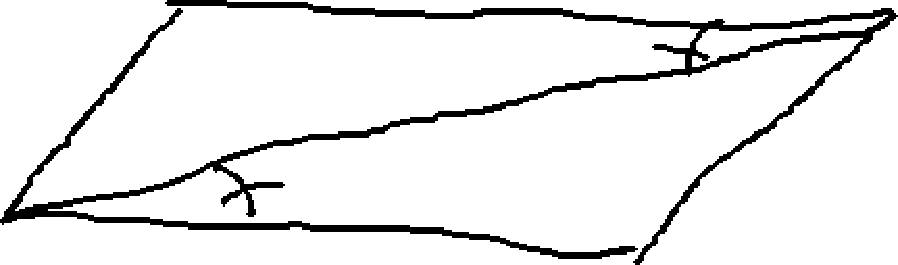
\includegraphics[width=0.5\linewidth]{codage_parall1.pdf}      % Ce graphique est également utilisé dans exo2smath-0178

    Tracer une figure respectant les mêmes codages, mais qui ne soit pas pas un parallélogramme. Préciser quelles droites sont parallèles et quelles droites ne sont pas parallèles.

\corrref{2smath-0325}
\end{exercice}
